% Options for packages loaded elsewhere
\PassOptionsToPackage{unicode}{hyperref}
\PassOptionsToPackage{hyphens}{url}
%
\documentclass[
]{article}
\usepackage{lmodern}
\usepackage{amssymb,amsmath}
\usepackage{ifxetex,ifluatex}
\ifnum 0\ifxetex 1\fi\ifluatex 1\fi=0 % if pdftex
  \usepackage[T1]{fontenc}
  \usepackage[utf8]{inputenc}
  \usepackage{textcomp} % provide euro and other symbols
\else % if luatex or xetex
  \usepackage{unicode-math}
  \defaultfontfeatures{Scale=MatchLowercase}
  \defaultfontfeatures[\rmfamily]{Ligatures=TeX,Scale=1}
\fi
% Use upquote if available, for straight quotes in verbatim environments
\IfFileExists{upquote.sty}{\usepackage{upquote}}{}
\IfFileExists{microtype.sty}{% use microtype if available
  \usepackage[]{microtype}
  \UseMicrotypeSet[protrusion]{basicmath} % disable protrusion for tt fonts
}{}
\makeatletter
\@ifundefined{KOMAClassName}{% if non-KOMA class
  \IfFileExists{parskip.sty}{%
    \usepackage{parskip}
  }{% else
    \setlength{\parindent}{0pt}
    \setlength{\parskip}{6pt plus 2pt minus 1pt}}
}{% if KOMA class
  \KOMAoptions{parskip=half}}
\makeatother
\usepackage{xcolor}
\IfFileExists{xurl.sty}{\usepackage{xurl}}{} % add URL line breaks if available
\IfFileExists{bookmark.sty}{\usepackage{bookmark}}{\usepackage{hyperref}}
\hypersetup{
  pdftitle={Taller Evaluable 1 2020, FIFA 2019},
  pdfauthor={mat3: Laura ; Lidia},
  hidelinks,
  pdfcreator={LaTeX via pandoc}}
\urlstyle{same} % disable monospaced font for URLs
\usepackage[margin=1in]{geometry}
\usepackage{color}
\usepackage{fancyvrb}
\newcommand{\VerbBar}{|}
\newcommand{\VERB}{\Verb[commandchars=\\\{\}]}
\DefineVerbatimEnvironment{Highlighting}{Verbatim}{commandchars=\\\{\}}
% Add ',fontsize=\small' for more characters per line
\usepackage{framed}
\definecolor{shadecolor}{RGB}{248,248,248}
\newenvironment{Shaded}{\begin{snugshade}}{\end{snugshade}}
\newcommand{\AlertTok}[1]{\textcolor[rgb]{0.94,0.16,0.16}{#1}}
\newcommand{\AnnotationTok}[1]{\textcolor[rgb]{0.56,0.35,0.01}{\textbf{\textit{#1}}}}
\newcommand{\AttributeTok}[1]{\textcolor[rgb]{0.77,0.63,0.00}{#1}}
\newcommand{\BaseNTok}[1]{\textcolor[rgb]{0.00,0.00,0.81}{#1}}
\newcommand{\BuiltInTok}[1]{#1}
\newcommand{\CharTok}[1]{\textcolor[rgb]{0.31,0.60,0.02}{#1}}
\newcommand{\CommentTok}[1]{\textcolor[rgb]{0.56,0.35,0.01}{\textit{#1}}}
\newcommand{\CommentVarTok}[1]{\textcolor[rgb]{0.56,0.35,0.01}{\textbf{\textit{#1}}}}
\newcommand{\ConstantTok}[1]{\textcolor[rgb]{0.00,0.00,0.00}{#1}}
\newcommand{\ControlFlowTok}[1]{\textcolor[rgb]{0.13,0.29,0.53}{\textbf{#1}}}
\newcommand{\DataTypeTok}[1]{\textcolor[rgb]{0.13,0.29,0.53}{#1}}
\newcommand{\DecValTok}[1]{\textcolor[rgb]{0.00,0.00,0.81}{#1}}
\newcommand{\DocumentationTok}[1]{\textcolor[rgb]{0.56,0.35,0.01}{\textbf{\textit{#1}}}}
\newcommand{\ErrorTok}[1]{\textcolor[rgb]{0.64,0.00,0.00}{\textbf{#1}}}
\newcommand{\ExtensionTok}[1]{#1}
\newcommand{\FloatTok}[1]{\textcolor[rgb]{0.00,0.00,0.81}{#1}}
\newcommand{\FunctionTok}[1]{\textcolor[rgb]{0.00,0.00,0.00}{#1}}
\newcommand{\ImportTok}[1]{#1}
\newcommand{\InformationTok}[1]{\textcolor[rgb]{0.56,0.35,0.01}{\textbf{\textit{#1}}}}
\newcommand{\KeywordTok}[1]{\textcolor[rgb]{0.13,0.29,0.53}{\textbf{#1}}}
\newcommand{\NormalTok}[1]{#1}
\newcommand{\OperatorTok}[1]{\textcolor[rgb]{0.81,0.36,0.00}{\textbf{#1}}}
\newcommand{\OtherTok}[1]{\textcolor[rgb]{0.56,0.35,0.01}{#1}}
\newcommand{\PreprocessorTok}[1]{\textcolor[rgb]{0.56,0.35,0.01}{\textit{#1}}}
\newcommand{\RegionMarkerTok}[1]{#1}
\newcommand{\SpecialCharTok}[1]{\textcolor[rgb]{0.00,0.00,0.00}{#1}}
\newcommand{\SpecialStringTok}[1]{\textcolor[rgb]{0.31,0.60,0.02}{#1}}
\newcommand{\StringTok}[1]{\textcolor[rgb]{0.31,0.60,0.02}{#1}}
\newcommand{\VariableTok}[1]{\textcolor[rgb]{0.00,0.00,0.00}{#1}}
\newcommand{\VerbatimStringTok}[1]{\textcolor[rgb]{0.31,0.60,0.02}{#1}}
\newcommand{\WarningTok}[1]{\textcolor[rgb]{0.56,0.35,0.01}{\textbf{\textit{#1}}}}
\usepackage{graphicx,grffile}
\makeatletter
\def\maxwidth{\ifdim\Gin@nat@width>\linewidth\linewidth\else\Gin@nat@width\fi}
\def\maxheight{\ifdim\Gin@nat@height>\textheight\textheight\else\Gin@nat@height\fi}
\makeatother
% Scale images if necessary, so that they will not overflow the page
% margins by default, and it is still possible to overwrite the defaults
% using explicit options in \includegraphics[width, height, ...]{}
\setkeys{Gin}{width=\maxwidth,height=\maxheight,keepaspectratio}
% Set default figure placement to htbp
\makeatletter
\def\fps@figure{htbp}
\makeatother
\setlength{\emergencystretch}{3em} % prevent overfull lines
\providecommand{\tightlist}{%
  \setlength{\itemsep}{0pt}\setlength{\parskip}{0pt}}
\setcounter{secnumdepth}{-\maxdimen} % remove section numbering

\title{Taller Evaluable 1 2020, FIFA 2019}
\author{mat3: Laura ; Lidia}
\date{3/12/2020}

\begin{document}
\maketitle

\hypertarget{taller-evaluable-datos-fifa-2020}{%
\section{Taller evaluable datos FIFA
2020}\label{taller-evaluable-datos-fifa-2020}}

Registraros en kaggle y bajaros el data set
\href{https://www.kaggle.com/stefanoleone992/fifa-20-complete-player-dataset}{FIFA
2020 Datos completos 2015 a 2020}. Guarda los datos en una carpeta
FIFA2020.

Las siguientes preguntas son relativas al data set
\texttt{players\_20.csv}.

Hay que contestar con código R explicar muy brevemente cada salida.
Subid a la activada el Rmd y el html.

En el mismo grupo de 3 que el proyecto final.

Rellenad estos datos:

** NOMBRE DEL GRUPO**

\begin{itemize}
\tightlist
\item
  Apellidos, Nombre Alumno1
\item
  Apellidos, Nombre Alumno1
\item
  Apellidos, Nombre Alumno1
\end{itemize}

\hypertarget{pregunta-0}{%
\subsection{Pregunta 0}\label{pregunta-0}}

Explica el data set y de qué tipo son cada una de las variables y en qué
tipo de fichero están guardadas. Carga los datos en un data frame con
\texttt{read.csv} y explica las clases de cada columna de datos. Explica
el parámeto \texttt{encoding}.

\begin{Shaded}
\begin{Highlighting}[]
\NormalTok{datos =}\StringTok{ }\KeywordTok{read.csv}\NormalTok{(}\StringTok{"FIFA2020/players_20.csv"}\NormalTok{, }\DataTypeTok{encoding=}\StringTok{"UTF-8"}\NormalTok{)}
\KeywordTok{head}\NormalTok{(datos, }\DecValTok{5}\NormalTok{)}
\end{Highlighting}
\end{Shaded}

\begin{verbatim}
##   sofifa_id
## 1    158023
## 2     20801
## 3    190871
## 4    200389
## 5    183277
##                                                              player_url
## 1               https://sofifa.com/player/158023/lionel-messi/20/159586
## 2 https://sofifa.com/player/20801/c-ronaldo-dos-santos-aveiro/20/159586
## 3  https://sofifa.com/player/190871/neymar-da-silva-santos-jr/20/159586
## 4                  https://sofifa.com/player/200389/jan-oblak/20/159586
## 5                https://sofifa.com/player/183277/eden-hazard/20/159586
##          short_name                           long_name age        dob
## 1          L. Messi      Lionel Andrés Messi Cuccittini  32 1987-06-24
## 2 Cristiano Ronaldo Cristiano Ronaldo dos Santos Aveiro  34 1985-02-05
## 3         Neymar Jr       Neymar da Silva Santos Junior  27 1992-02-05
## 4          J. Oblak                           Jan Oblak  26 1993-01-07
## 5         E. Hazard                         Eden Hazard  28 1991-01-07
##   height_cm weight_kg nationality                club overall potential
## 1       170        72   Argentina        FC Barcelona      94        94
## 2       187        83    Portugal            Juventus      93        93
## 3       175        68      Brazil Paris Saint-Germain      92        92
## 4       188        87    Slovenia     Atlético Madrid      91        93
## 5       175        74     Belgium         Real Madrid      91        91
##   value_eur wage_eur player_positions preferred_foot international_reputation
## 1  95500000   565000       RW, CF, ST           Left                        5
## 2  58500000   405000           ST, LW          Right                        5
## 3 105500000   290000          LW, CAM          Right                        5
## 4  77500000   125000               GK          Right                        3
## 5  90000000   470000           LW, CF          Right                        4
##   weak_foot skill_moves     work_rate  body_type real_face release_clause_eur
## 1         4           4    Medium/Low      Messi       Yes          195800000
## 2         4           5      High/Low C. Ronaldo       Yes           96500000
## 3         5           5   High/Medium     Neymar       Yes          195200000
## 4         3           1 Medium/Medium     Normal       Yes          164700000
## 5         4           4   High/Medium     Normal       Yes          184500000
##                                                                                                                            player_tags
## 1                              #Dribbler, #Distance Shooter, #Crosser, #FK Specialist, #Acrobat, #Clinical Finisher, #Complete Forward
## 2                                            #Speedster, #Dribbler, #Distance Shooter, #Acrobat, #Clinical Finisher, #Complete Forward
## 3 #Speedster, #Dribbler, #Playmaker  , #Crosser, #FK Specialist, #Acrobat, #Clinical Finisher, #Complete Midfielder, #Complete Forward
## 4                                                                                                                                     
## 5                                                                                                      #Speedster, #Dribbler, #Acrobat
##   team_position team_jersey_number loaned_from     joined contract_valid_until
## 1            RW                 10             2004-07-01                 2021
## 2            LW                  7             2018-07-10                 2022
## 3           CAM                 10             2017-08-03                 2022
## 4            GK                 13             2014-07-16                 2023
## 5            LW                  7             2019-07-01                 2024
##   nation_position nation_jersey_number pace shooting passing dribbling
## 1                                   NA   87       92      92        96
## 2              LS                    7   90       93      82        89
## 3              LW                   10   91       85      87        95
## 4              GK                    1   NA       NA      NA        NA
## 5              LF                   10   91       83      86        94
##   defending physic gk_diving gk_handling gk_kicking gk_reflexes gk_speed
## 1        39     66        NA          NA         NA          NA       NA
## 2        35     78        NA          NA         NA          NA       NA
## 3        32     58        NA          NA         NA          NA       NA
## 4        NA     NA        87          92         78          89       52
## 5        35     66        NA          NA         NA          NA       NA
##   gk_positioning
## 1             NA
## 2             NA
## 3             NA
## 4             90
## 5             NA
##                                                                                                                                         player_traits
## 1 Beat Offside Trap, Argues with Officials, Early Crosser, Finesse Shot, Speed Dribbler (CPU AI Only), 1-on-1 Rush, Giant Throw-in, Outside Foot Shot
## 2                                       Long Throw-in, Selfish, Argues with Officials, Early Crosser, Speed Dribbler (CPU AI Only), Skilled Dribbling
## 3                                                 Power Free-Kick, Injury Free, Selfish, Early Crosser, Speed Dribbler (CPU AI Only), Crowd Favourite
## 4                                                                                                                          Flair, Acrobatic Clearance
## 5                                                             Beat Offside Trap, Selfish, Finesse Shot, Speed Dribbler (CPU AI Only), Crowd Favourite
##   attacking_crossing attacking_finishing attacking_heading_accuracy
## 1                 88                  95                         70
## 2                 84                  94                         89
## 3                 87                  87                         62
## 4                 13                  11                         15
## 5                 81                  84                         61
##   attacking_short_passing attacking_volleys skill_dribbling skill_curve
## 1                      92                88              97          93
## 2                      83                87              89          81
## 3                      87                87              96          88
## 4                      43                13              12          13
## 5                      89                83              95          83
##   skill_fk_accuracy skill_long_passing skill_ball_control movement_acceleration
## 1                94                 92                 96                    91
## 2                76                 77                 92                    89
## 3                87                 81                 95                    94
## 4                14                 40                 30                    43
## 5                79                 83                 94                    94
##   movement_sprint_speed movement_agility movement_reactions movement_balance
## 1                    84               93                 95               95
## 2                    91               87                 96               71
## 3                    89               96                 92               84
## 4                    60               67                 88               49
## 5                    88               95                 90               94
##   power_shot_power power_jumping power_stamina power_strength power_long_shots
## 1               86            68            75             68               94
## 2               95            95            85             78               93
## 3               80            61            81             49               84
## 4               59            78            41             78               12
## 5               82            56            84             63               80
##   mentality_aggression mentality_interceptions mentality_positioning
## 1                   48                      40                    94
## 2                   63                      29                    95
## 3                   51                      36                    87
## 4                   34                      19                    11
## 5                   54                      41                    87
##   mentality_vision mentality_penalties mentality_composure defending_marking
## 1               94                  75                  96                33
## 2               82                  85                  95                28
## 3               90                  90                  94                27
## 4               65                  11                  68                27
## 5               89                  88                  91                34
##   defending_standing_tackle defending_sliding_tackle goalkeeping_diving
## 1                        37                       26                  6
## 2                        32                       24                  7
## 3                        26                       29                  9
## 4                        12                       18                 87
## 5                        27                       22                 11
##   goalkeeping_handling goalkeeping_kicking goalkeeping_positioning
## 1                   11                  15                      14
## 2                   11                  15                      14
## 3                    9                  15                      15
## 4                   92                  78                      90
## 5                   12                   6                       8
##   goalkeeping_reflexes   ls   st   rs   lw   lf   cf   rf   rw  lam  cam  ram
## 1                    8 89+2 89+2 89+2 93+2 93+2 93+2 93+2 93+2 93+2 93+2 93+2
## 2                   11 91+3 91+3 91+3 89+3 90+3 90+3 90+3 89+3 88+3 88+3 88+3
## 3                   11 84+3 84+3 84+3 90+3 89+3 89+3 89+3 90+3 90+3 90+3 90+3
## 4                   89                                                       
## 5                    8 83+3 83+3 83+3 89+3 88+3 88+3 88+3 89+3 89+3 89+3 89+3
##     lm  lcm   cm  rcm   rm  lwb  ldm  cdm  rdm  rwb   lb  lcb   cb  rcb   rb
## 1 92+2 87+2 87+2 87+2 92+2 68+2 66+2 66+2 66+2 68+2 63+2 52+2 52+2 52+2 63+2
## 2 88+3 81+3 81+3 81+3 88+3 65+3 61+3 61+3 61+3 65+3 61+3 53+3 53+3 53+3 61+3
## 3 89+3 82+3 82+3 82+3 89+3 66+3 61+3 61+3 61+3 66+3 61+3 46+3 46+3 46+3 61+3
## 4                                                                           
## 5 89+3 83+3 83+3 83+3 89+3 66+3 63+3 63+3 63+3 66+3 61+3 49+3 49+3 49+3 61+3
\end{verbatim}

\hypertarget{pregunta-1}{%
\subsection{Pregunta 1}\label{pregunta-1}}

¿Qué clubs tienen a los 10 mejores jugadores según su ``overall''?

\begin{Shaded}
\begin{Highlighting}[]
\NormalTok{sort_overall =}\KeywordTok{sort}\NormalTok{(datos}\OperatorTok{$}\NormalTok{overall,}\DataTypeTok{decreasing=}\OtherTok{TRUE}\NormalTok{)[}\DecValTok{1}\OperatorTok{:}\DecValTok{10}\NormalTok{]}
\NormalTok{clubs =}\StringTok{ }\NormalTok{datos[datos}\OperatorTok{$}\NormalTok{overall }\OperatorTok\StringTok{ }\NormalTok{sort_overall,]}\OperatorTok{$}\NormalTok{club}
\NormalTok{clubs =}\StringTok{ }\KeywordTok{as.vector}\NormalTok{(clubs)}
\NormalTok{clubs =}\StringTok{ }\NormalTok{clubs[}\OperatorTok{!}\KeywordTok{duplicated}\NormalTok{(clubs)]}
\end{Highlighting}
\end{Shaded}

\begin{Shaded}
\begin{Highlighting}[]
\NormalTok{clubs =}\StringTok{ }\NormalTok{datos[}\KeywordTok{order}\NormalTok{(datos}\OperatorTok{$}\NormalTok{overall, }\DataTypeTok{decreasing=}\OtherTok{TRUE}\NormalTok{)[}\DecValTok{1}\OperatorTok{:}\DecValTok{10}\NormalTok{], }\StringTok{"club"}\NormalTok{]}
\NormalTok{clubs =}\StringTok{ }\KeywordTok{unique}\NormalTok{(clubs)}
\NormalTok{clubs}
\end{Highlighting}
\end{Shaded}

\begin{verbatim}
## [1] FC Barcelona        Juventus            Paris Saint-Germain
## [4] Atlético Madrid     Real Madrid         Manchester City    
## [7] Liverpool          
## 698 Levels:  SSV Jahn Regensburg 1. FC Heidenheim 1846 ... Zaglebie Lubin
\end{verbatim}

\hypertarget{pregunta-2}{%
\subsection{Pregunta 2}\label{pregunta-2}}

Crea un dataframe ``sub\_fifa20'' que contenga a los jugadores de los
clubs encontrados en el ejercicio anterior.

\begin{Shaded}
\begin{Highlighting}[]
\NormalTok{sub_fifa20 =datos[datos}\OperatorTok{$}\NormalTok{club }\OperatorTok\StringTok{ }\NormalTok{clubs, ]}
\end{Highlighting}
\end{Shaded}

\hypertarget{pregunta-3}{%
\subsection{Pregunta 3}\label{pregunta-3}}

Calcula la media y desviación típica muestral de los sueldos de los
jugadores por equipo del dataframe sub\_fifa20.

\begin{Shaded}
\begin{Highlighting}[]
\KeywordTok{aggregate}\NormalTok{(wage_eur}\OperatorTok{~}\NormalTok{club,}\DataTypeTok{data=}\NormalTok{sub_fifa20,}\DataTypeTok{FUN=} \ControlFlowTok{function}\NormalTok{(x) \{}\KeywordTok{c}\NormalTok{(}\DataTypeTok{media=}\KeywordTok{mean}\NormalTok{(x),}\DataTypeTok{sd=}\KeywordTok{sd}\NormalTok{(x))\})}
\end{Highlighting}
\end{Shaded}

\begin{verbatim}
##                  club wage_eur.media wage_eur.sd
## 1     Atlético Madrid       44848.48    31608.07
## 2        FC Barcelona      150000.00   130914.81
## 3            Juventus      113636.36    77462.42
## 4           Liverpool       80818.18    67478.91
## 5     Manchester City      120727.27    99257.01
## 6 Paris Saint-Germain       72606.06    65992.40
## 7         Real Madrid      162242.42   111794.46
\end{verbatim}

\begin{Shaded}
\begin{Highlighting}[]
\NormalTok{f =}\StringTok{ }\ControlFlowTok{function}\NormalTok{(x) \{}\KeywordTok{c}\NormalTok{(}\KeywordTok{mean}\NormalTok{(x),}\KeywordTok{sd}\NormalTok{(x))\}}
\NormalTok{tabla =}\StringTok{ }\KeywordTok{aggregate}\NormalTok{(wage_eur}\OperatorTok{~}\NormalTok{club,}\DataTypeTok{data=}\NormalTok{sub_fifa20,}\DataTypeTok{FUN=}\NormalTok{f)}
\NormalTok{tabla2 =}\StringTok{ }\KeywordTok{data.frame}\NormalTok{(}\DataTypeTok{Club=}\NormalTok{tabla}\OperatorTok{$}\NormalTok{club, }\DataTypeTok{Sueldo_medio =}\NormalTok{ tabla}\OperatorTok{$}\NormalTok{wage_eur[, }\DecValTok{1}\NormalTok{], }\DataTypeTok{Desv_tip_mues =}\NormalTok{ tabla}\OperatorTok{$}\NormalTok{wage_eur[, }\DecValTok{2}\NormalTok{])}
\NormalTok{tabla2}
\end{Highlighting}
\end{Shaded}

\begin{verbatim}
##                  Club Sueldo_medio Desv_tip_mues
## 1     Atlético Madrid     44848.48      31608.07
## 2        FC Barcelona    150000.00     130914.81
## 3            Juventus    113636.36      77462.42
## 4           Liverpool     80818.18      67478.91
## 5     Manchester City    120727.27      99257.01
## 6 Paris Saint-Germain     72606.06      65992.40
## 7         Real Madrid    162242.42     111794.46
\end{verbatim}

\hypertarget{pregunta-4}{%
\subsection{Pregunta 4}\label{pregunta-4}}

Discretiza la variable age de sub\_fifa20 en los 3 niveles siguientes:
``freshman'', ``junior'', ``senior'', según los cortes por defecto. La
variable resultante age\_Level tiene que ser un factor ordenado en orden
creciente de edad.

\begin{Shaded}
\begin{Highlighting}[]
\NormalTok{age_Level=}\KeywordTok{ordered}\NormalTok{(}\KeywordTok{cut}\NormalTok{(sub_fifa20}\OperatorTok{$}\NormalTok{age,}\DataTypeTok{breaks=}\DecValTok{3}\NormalTok{),}\DataTypeTok{labels=}\KeywordTok{c}\NormalTok{(}\StringTok{"freshman"}\NormalTok{,}\StringTok{"junior"}\NormalTok{,}\StringTok{"senior"}\NormalTok{))}
\KeywordTok{head}\NormalTok{(age_Level)}
\end{Highlighting}
\end{Shaded}

\begin{verbatim}
## [1] junior senior junior junior junior junior
## Levels: freshman < junior < senior
\end{verbatim}

\hypertarget{pregunta-5}{%
\subsection{Pregunta 5}\label{pregunta-5}}

¿Qué club tiene a más jugadores en el nivel ``freshman'' calculado en el
ejercicio anterior?

\begin{Shaded}
\begin{Highlighting}[]
\NormalTok{sub_fifa20}\OperatorTok{$}\NormalTok{age_level =}\StringTok{ }\NormalTok{age_Level}
\KeywordTok{aggregate}\NormalTok{(age_level}\OperatorTok{~}\NormalTok{club,}\DataTypeTok{data=}\NormalTok{sub_fifa20,}\DataTypeTok{FUN=}\ControlFlowTok{function}\NormalTok{(x) }\KeywordTok{sum}\NormalTok{(x}\OperatorTok{==}\StringTok{'freshman'}\NormalTok{))}
\end{Highlighting}
\end{Shaded}

\begin{verbatim}
##                  club age_level
## 1     Atlético Madrid        19
## 2        FC Barcelona        21
## 3            Juventus        14
## 4           Liverpool        18
## 5     Manchester City        23
## 6 Paris Saint-Germain        19
## 7         Real Madrid        16
\end{verbatim}

\begin{Shaded}
\begin{Highlighting}[]
\KeywordTok{aggregate}\NormalTok{(age_level}\OperatorTok{~}\NormalTok{club,}\DataTypeTok{data=}\NormalTok{sub_fifa20,}\DataTypeTok{FUN=}\ControlFlowTok{function}\NormalTok{(x) }\KeywordTok{table}\NormalTok{(x)[}\StringTok{"freshman"}\NormalTok{] )}
\end{Highlighting}
\end{Shaded}

\begin{verbatim}
##                  club age_level
## 1     Atlético Madrid        19
## 2        FC Barcelona        21
## 3            Juventus        14
## 4           Liverpool        18
## 5     Manchester City        23
## 6 Paris Saint-Germain        19
## 7         Real Madrid        16
\end{verbatim}

\hypertarget{pregunta-6}{%
\subsection{Pregunta 6}\label{pregunta-6}}

¿Cuántas nacionalidades hay entre todos los jugadores de sub\_fifa20?
¿Qué club tiene mayor cantidad de nacionalidades?

\begin{Shaded}
\begin{Highlighting}[]
\KeywordTok{length}\NormalTok{(}\KeywordTok{unique}\NormalTok{(sub_fifa20}\OperatorTok{$}\NormalTok{nationality))}
\end{Highlighting}
\end{Shaded}

\begin{verbatim}
## [1] 36
\end{verbatim}

\begin{Shaded}
\begin{Highlighting}[]
\NormalTok{nationalities_per_club =}\StringTok{ }\KeywordTok{aggregate}\NormalTok{(nationality}\OperatorTok{~}\NormalTok{club,}\DataTypeTok{data=}\NormalTok{sub_fifa20,}\DataTypeTok{FUN=}\ControlFlowTok{function}\NormalTok{(x) }\KeywordTok{length}\NormalTok{(}\KeywordTok{unique}\NormalTok{(x)))}
\NormalTok{nationalities_per_club[nationalities_per_club}\OperatorTok{$}\NormalTok{nationality}\OperatorTok{==}\KeywordTok{max}\NormalTok{(nationalities_per_club}\OperatorTok{$}\NormalTok{nationality),]}
\end{Highlighting}
\end{Shaded}

\begin{verbatim}
##              club nationality
## 1 Atlético Madrid          15
## 4       Liverpool          15
\end{verbatim}

\hypertarget{pregunta-7}{%
\subsection{Pregunta 7}\label{pregunta-7}}

Calcula mediante un diagrama de tarta la proporción de jugadores de cada
nacionalidad en cada club

\begin{Shaded}
\begin{Highlighting}[]
\ControlFlowTok{for}\NormalTok{(club }\ControlFlowTok{in}\NormalTok{ clubs)\{}
\NormalTok{  nationalities =}\StringTok{ }\NormalTok{sub_fifa20[sub_fifa20}\OperatorTok{$}\NormalTok{club }\OperatorTok\StringTok{ }\KeywordTok{c}\NormalTok{(club), ]}\OperatorTok{$}\NormalTok{nationality}
\NormalTok{  nationalities =}\StringTok{ }\KeywordTok{as.vector}\NormalTok{(nationalities)}
  \KeywordTok{pie}\NormalTok{(}\KeywordTok{table}\NormalTok{(nationalities), }\DataTypeTok{main=}\KeywordTok{paste0}\NormalTok{(}\StringTok{"Proporción de nacionalidades en el"}\NormalTok{, club))}
\NormalTok{\}}
\end{Highlighting}
\end{Shaded}

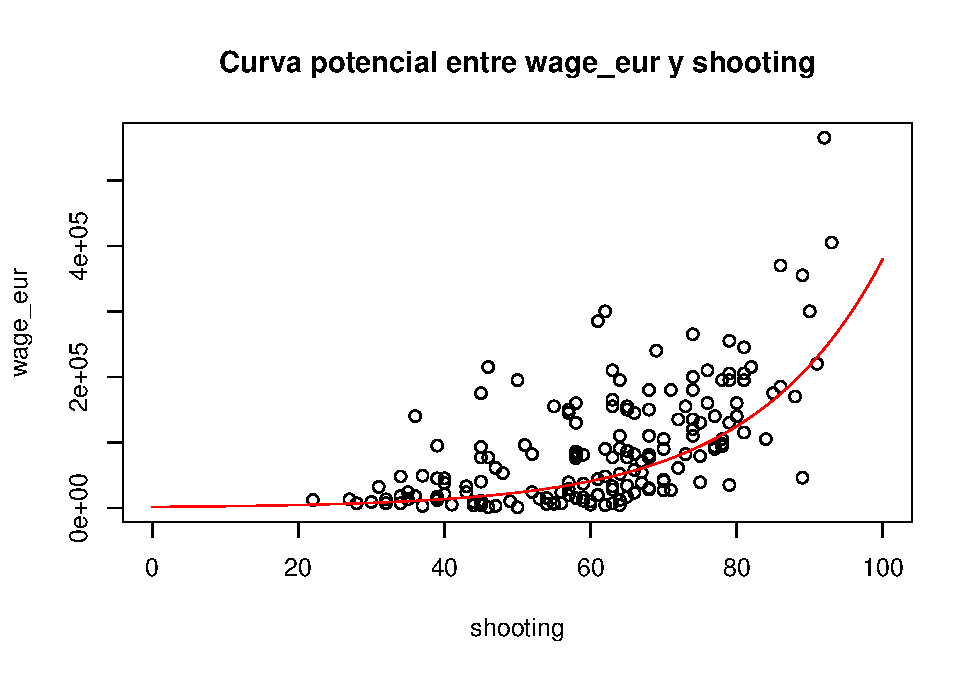
\includegraphics{taller_evaluable1_files/figure-latex/unnamed-chunk-12-1.pdf}
\includegraphics{taller_evaluable1_files/figure-latex/unnamed-chunk-12-2.pdf}
\includegraphics{taller_evaluable1_files/figure-latex/unnamed-chunk-12-3.pdf}
\includegraphics{taller_evaluable1_files/figure-latex/unnamed-chunk-12-4.pdf}
\includegraphics{taller_evaluable1_files/figure-latex/unnamed-chunk-12-5.pdf}
\includegraphics{taller_evaluable1_files/figure-latex/unnamed-chunk-12-6.pdf}
\includegraphics{taller_evaluable1_files/figure-latex/unnamed-chunk-12-7.pdf}

\begin{Shaded}
\begin{Highlighting}[]
\KeywordTok{aggregate}\NormalTok{(nationality}\OperatorTok{~}\NormalTok{club, sub_fifa20, }\DataTypeTok{FUN =}\ControlFlowTok{function}\NormalTok{(x) }\KeywordTok{pie}\NormalTok{(}\KeywordTok{table}\NormalTok{(}\KeywordTok{droplevels}\NormalTok{(x))))}
\end{Highlighting}
\end{Shaded}

\includegraphics{taller_evaluable1_files/figure-latex/unnamed-chunk-13-1.pdf}
\includegraphics{taller_evaluable1_files/figure-latex/unnamed-chunk-13-2.pdf}
\includegraphics{taller_evaluable1_files/figure-latex/unnamed-chunk-13-3.pdf}
\includegraphics{taller_evaluable1_files/figure-latex/unnamed-chunk-13-4.pdf}
\includegraphics{taller_evaluable1_files/figure-latex/unnamed-chunk-13-5.pdf}
\includegraphics{taller_evaluable1_files/figure-latex/unnamed-chunk-13-6.pdf}
\includegraphics{taller_evaluable1_files/figure-latex/unnamed-chunk-13-7.pdf}

\begin{verbatim}
##                  club nationality
## 1     Atlético Madrid        NULL
## 2        FC Barcelona        NULL
## 3            Juventus        NULL
## 4           Liverpool        NULL
## 5     Manchester City        NULL
## 6 Paris Saint-Germain        NULL
## 7         Real Madrid        NULL
\end{verbatim}

\hypertarget{pregunta-8}{%
\subsection{Pregunta 8}\label{pregunta-8}}

Encuentra la función (lineal, exponencial o potencial) que mejor
describe la dependencia funcional del sueldo de los jugadores en función
de la variable overall en el dataframe sub\_fifa20. Representa dicha
función junto con los puntos (overall, sueldo) en escala lineal.

\begin{Shaded}
\begin{Highlighting}[]
\KeywordTok{summary}\NormalTok{(}\KeywordTok{lm}\NormalTok{(sub_fifa20}\OperatorTok{$}\NormalTok{wage_eur}\OperatorTok{~}\NormalTok{sub_fifa20}\OperatorTok{$}\NormalTok{overall))}\OperatorTok{$}\NormalTok{r.squared}
\end{Highlighting}
\end{Shaded}

\begin{verbatim}
## [1] 0.657717
\end{verbatim}

\begin{Shaded}
\begin{Highlighting}[]
\KeywordTok{summary}\NormalTok{(}\KeywordTok{lm}\NormalTok{(}\KeywordTok{log10}\NormalTok{(sub_fifa20}\OperatorTok{$}\NormalTok{wage_eur)}\OperatorTok{~}\NormalTok{sub_fifa20}\OperatorTok{$}\NormalTok{overall))}\OperatorTok{$}\NormalTok{r.squared}
\end{Highlighting}
\end{Shaded}

\begin{verbatim}
## [1] 0.8816264
\end{verbatim}

\begin{Shaded}
\begin{Highlighting}[]
\KeywordTok{summary}\NormalTok{(}\KeywordTok{lm}\NormalTok{(}\KeywordTok{log10}\NormalTok{(sub_fifa20}\OperatorTok{$}\NormalTok{wage_eur)}\OperatorTok{~}\KeywordTok{log10}\NormalTok{(sub_fifa20}\OperatorTok{$}\NormalTok{overall)))}\OperatorTok{$}\NormalTok{r.squared}
\end{Highlighting}
\end{Shaded}

\begin{verbatim}
## [1] 0.8859737
\end{verbatim}

\begin{Shaded}
\begin{Highlighting}[]
\KeywordTok{lm}\NormalTok{(}\KeywordTok{log10}\NormalTok{(sub_fifa20}\OperatorTok{$}\NormalTok{wage_eur)}\OperatorTok{~}\KeywordTok{log10}\NormalTok{(sub_fifa20}\OperatorTok{$}\NormalTok{overall))}
\end{Highlighting}
\end{Shaded}

\begin{verbatim}
## 
## Call:
## lm(formula = log10(sub_fifa20$wage_eur) ~ log10(sub_fifa20$overall))
## 
## Coefficients:
##               (Intercept)  log10(sub_fifa20$overall)  
##                    -14.29                      10.10
\end{verbatim}

\[
\textrm{wage_eur}(\textrm{overall}) = 10^{-14.29} \cdot \textrm{overall}^{10.10}
\]

\begin{Shaded}
\begin{Highlighting}[]
\KeywordTok{plot}\NormalTok{(sub_fifa20}\OperatorTok{$}\NormalTok{overall, sub_fifa20}\OperatorTok{$}\NormalTok{wage_eur)}
\KeywordTok{curve}\NormalTok{(}\DecValTok{10}\OperatorTok{^-}\FloatTok{14.29}\OperatorTok{*}\NormalTok{x}\OperatorTok{^}\FloatTok{10.10}\NormalTok{, }\DataTypeTok{add =} \OtherTok{TRUE}\NormalTok{, }\DataTypeTok{col=}\StringTok{"red"}\NormalTok{)}
\end{Highlighting}
\end{Shaded}

\includegraphics{taller_evaluable1_files/figure-latex/unnamed-chunk-16-1.pdf}

\end{document}
